\documentclass{beamer}
\usepackage[utf8]{inputenc}
\usepackage{default}
\usepackage{multirow} 
\usepackage{amsmath} 
\usepackage{listings}

\lstset{ %
                % choose the language of the code
basicstyle=\footnotesize,       % the size of the fonts that are used for the code
numbers=left,                   % where to put the line-numbers
numberstyle=\footnotesize,      % the size of the fonts that are used for the line-numbers
stepnumber=1,                   % the step between two line-numbers. If it is 1 each line will be numbered
numbersep=5pt,                  % how far the line-numbers are from the code
backgroundcolor=\color{white},  % choose the background color. You must add \usepackage{color}
showspaces=false,               % show spaces adding particular underscores
showstringspaces=false,         % underline spaces within strings
showtabs=false,                 % show tabs within strings adding particular underscores
frame=single,           % adds a frame around the code
tabsize=2,          % sets default tabsize to 2 spaces
captionpos=b,           % sets the caption-position to bottom
breaklines=true,        % sets automatic line breaking
breakatwhitespace=false,    % sets if automatic breaks should only happen at whitespace
escapeinside={\%*}{*)}          % if you want to add a comment within your code
}

\usetheme{Berkeley}

\title{Subprogramas}
\author{Guilherme, Gustavo, Sean e Vinícius}
\institute{Universidade Estadual de Londrina}

\begin{document}

\frame{\titlepage}
\frame {
\frametitle{Sumário}
\tableofcontents
}

\section{Ambiente de referênciamento locais}
\begin{frame}{Ambiente de referênciamento locais}
\begin{block}{Variáveis locais estáticas}
	São vinculadas ao armazenamento antes da execução do programa e continuam até seu término.
	\begin{itemize}
	  \item + Endereçamento direto na memória.
	  \item + Não causam sobrecarga na alocação e desalocação.
	  \item - Não se comportam bem em programas recursivos.
	  \item - Representam um estado global.
	\end{itemize}
\end{block}
\end{frame}

\begin{frame}{Ambiente de referênciamento locais}
\begin{figure}[ht!]
 \centering
 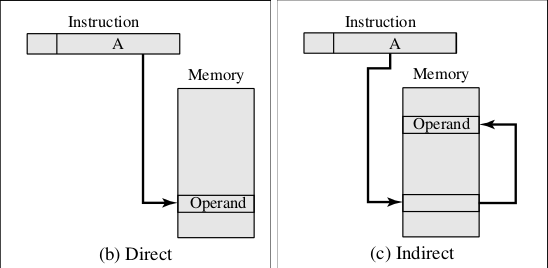
\includegraphics[scale=0.5]{./imgs/enderecamento.png}
\label{enderecamento}
\end{figure}
\end{frame}

\begin{frame}[fragile]{Ambiente de referênciamento locais}
\begin{lstlisting}
int sum (int arr[], int n)
{
    static int result = 0;
    if (n == 0)
        return result ;
    else {
        result += arr[n - 1];
        sum(arr, n - 1);
     }
}

int main(void) {
    int array[5] = {1,2,3,4,5};
    printf("%d\n", sum(array, 3));  // 6
    printf("%d\n", sum(array, 3));  // 12
    printf("%d\n", sum(array, 3));  // 18
    return 0;
}
\end{lstlisting}
\end{frame}

\begin{frame}{Ambiente de referênciamento locais}
\begin{block}{Variáveis locais dinâmicas na pilha}
	Variáveis dinâmicas na pilha, são vinculadas ao armazenamento quando o subprograma inicia sua execução e desvinculadas do armazenamento quando ele se encerra.
	\begin{itemize}
	  \item + Maior flexibilidade (programas recursivos).
	  \item - Sobrecarga na alocação e desalocação.
	  \item - Endereçamento indireto.
	\end{itemize}
\end{block}
\end{frame}

\begin{frame}{Ambiente de referênciamento locais}
\begin{block}{Exemplos}
	\begin{itemize}
	  \item ALGOL 60 e suas linguagens descendentes, possuem variáveis locais dinâmicas na pilha.
	  \item Funções em C possuem variáveis são dinâmicas na pilha a menos que sejam especificamente declaradas como static. 
	  \item Subprogramas Pascal e Ada e métodos em C++, Java, C\# têm somente variaveis dinâmicas na pilha. 
	\end{itemize}
\end{block}
\end{frame}

\section{Aninhamento de subprogramas} 
\begin{frame}[fragile]{Aninhamento de subprogramas}
Linguagens como ALGOL 68, Pascal e Ada, JavaScript, Python e Lua permitem aninhamento de subprogramas. Linguagens descententes de C não permitem aninhamento.
\begin{verbatim}
function hipotenusa(a, b) {
   function quadrado(x) {
      return x * x; 
   }
   return Math.sqrt(quadrado(a) + quadrado(b));
}
\end{verbatim}
\end{frame} %sean
%!TEX root = slide.tex

\section{Subprogramas Como Parâmetro}
\begin{frame}{Subprogramas Como Parâmetro}
	\begin{itemize}
	  \item Ideia simples, mas gera complicações.
	  \item \emph{Type checking}.
	  \item referencing environment.
	\end{itemize}
\end{frame}

\begin{frame}{Referencing Environment}
	\begin{itemize}
	  \item Linguagens que permitem subprogramas aninhados.
	  \item Shallow Binding
	  \item Deep Binding
	  \item Ad Hoc Binding
	\end{itemize}
\end{frame}

\begin{frame}{Exemplo}
	\begin{figure}[ht!]
		\centering
		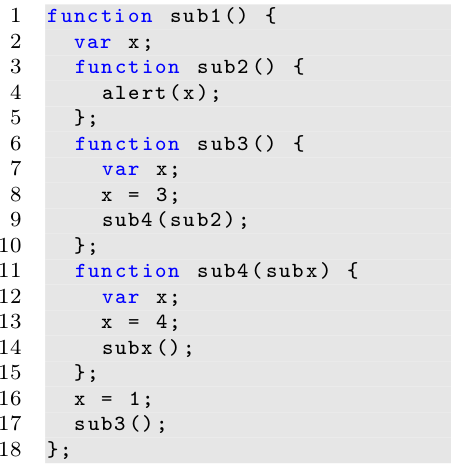
\includegraphics[scale=0.4]{./imgs/js-original}
	\end{figure}
\end{frame}

\begin{frame}{Shallow Binding}
	O ambiente é o local onde o subprograma é chamado.
\end{frame}

\begin{frame}{Shallow Binding}
	\begin{figure}[ht!]
		\centering
		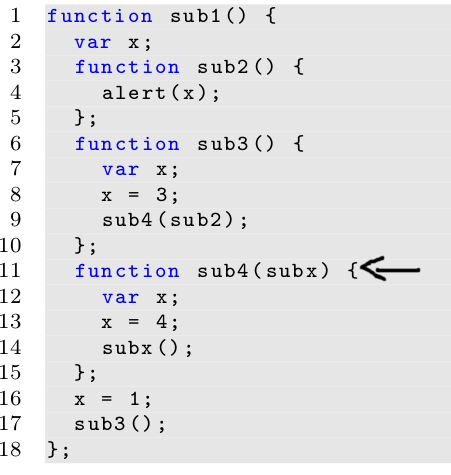
\includegraphics[scale=0.4]{./imgs/js-shallow}
	\end{figure}
\end{frame}

\begin{frame}{Deep Binding}
	O ambiente refere-se onde o subprograma foi definido.
\end{frame}

\begin{frame}{Deep Binding}
	\begin{figure}[ht!]
		\centering
		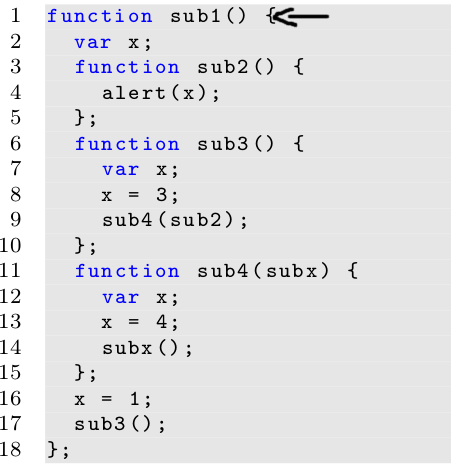
\includegraphics[scale=0.4]{./imgs/js-deep}
	\end{figure}
\end{frame}

\begin{frame}{Ad Hoc Binding}
	O ambiente condiz com o local que o subprograma foi passado por parâmetro.
	Nunca implementado.
\end{frame}

\begin{frame}{Ad Hoc Binding}
	\begin{figure}[ht!]
		\centering
		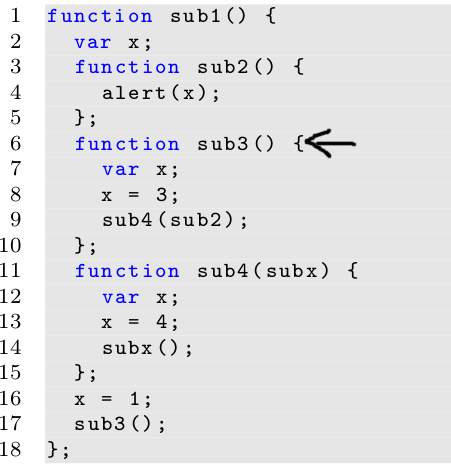
\includegraphics[scale=0.4]{./imgs/js-adhoc}
	\end{figure}
\end{frame}

\section{Chamar Subprogramas Indiretamente}
\begin{frame}{Chamar Subprogramas Indiretamente}
	\begin{itemize}
	  \item Subprograma conhecido em tempo de execução.
	  \item GUI e callback.
	  \item C/C++ ponteiro para função.
	  \item C\# Delegate.
	\end{itemize}
\end{frame}

\begin{frame}[fragile]{C/C++ - Ponteiro Para Função}
	\begin{lstlisting}[language=c]
		//declaracao da funcao
		int sum(int a, int b)
		{
			return a + b;
		}

		//ponteiro para a funcao
		int (*sum_pointer)(int, int);
		sum_pointer = &sum;
		
		//chamar a funcao
		(*sum_pointer)(1,2);
	\end{lstlisting}
\end{frame}

\begin{frame}[fragile]{C\# - Delegate}
	\begin{lstlisting}[language=csh]
		//declarar um delegate
		public delegate int SumDelegate(int a, int b);
		...
		//instanciar um delegate (funcao sum tem a mesma assinatura)
		SumDelegate sumDelegate = new SumDelegate(sum);
		//executar
		sumDelegate(2,3);
	\end{lstlisting}
\end{frame}

\section{Sobrecarga de Subprogramas}
\begin{frame}{Sobrecarga de Subprogramas}
	\begin{itemize}
	  \item Subprogramas (diferentes) com o mesmo nome.
	  \item Parâmetros diferentes.
	  \item Subprogramas relacionados.
	  \item Exemplo: Sobrecarga de construtor.
	  \item Ada, Java, C++, C\# e F\#.
	\end{itemize}
\end{frame}

\section{Suprogramas Genéricos}
\begin{frame}{Suprogramas Genéricos}
	\begin{itemize}
	  \item Reuso de software é algo importante.
	  \item Subprogramas com tipos genéricos.
	  \item Exemplo: Ordenação independente de tipo.
	  \item C++ - Templates
	  \item Java e C\# - Generics
	\end{itemize}
\end{frame}

\begin{frame}[fragile]{C++ - Templates}
	\begin{lstlisting}[language=c++]
		//declarar funcao template
		template <class myType>
			myType GetMax (myType a, myType b) {
			return (a>b?a:b);
		}
		...
		//exemplo de chamada para inteiro
		GetMax<int> (1,2);
		...
		//exemplo de chamada para float
		GetMax<float> (1,2);
	\end{lstlisting}
\end{frame}

\begin{frame}[fragile]{Java - Generics}
	\begin{lstlisting}[language=Java]
		//declarar um metodo generico.
		public static <T> T doIt(T[] list) {
			...
		}
		...
		//chamar o metodo para String
		doIt<String>(myList);
		
		...
		//chamar o metodo para Integer
		doIt<Integer>(myList);
		
		...
		//isso causaria um erro (tipo primitivo)
		doIt<int>(myList);
	\end{lstlisting}
\end{frame}
\section{Questões de projetos referente a funções}
\begin{frame}{Questões de projetos referente a funções}
\begin{block}{Considerações}
	\begin{itemize}
	  \item Efeitos colaterais
	  \item Tipos de valores retornados
	  \item Quantidade de valores retornados
	\end{itemize}
\end{block}
\end{frame}

\begin{frame}[fragile]{Efeitos colaterais}
\begin{block}{Exemplo de aliasing}
	\begin{verbatim}
		int x = 3; 
		... 
		... // se int* y = &x;
		*y = 9;
	\end{verbatim}
\end{block}
\end{frame}

\begin{frame}{Tipos de valores retornados}
\begin{block}{Alguns exemplos}
	\begin{itemize}
		\item C permite qualquer tipo ser retornado por suas funções exceto vetores e funções. 
		\item C++ permite tipos definidos pelo usuário ou classes serem retornados. 
		\item Java e C\#, qualquer tipo ou classe podem ser retornados por seus métodos.
	\end{itemize}
\end{block}
\end{frame}

\begin{frame}[fragile]{Quantidade de valores retornados}
\begin{block}{Linguagem Lua}
	Lua permite o retorno de múltiplos valores de suas funções. Por exemplo, a chamada da função:
	\begin{verbatim}
		a, b, c = fun() 
	\end{verbatim}
	Recebe três valores de retorno da função func():  
	\begin{verbatim}
		return 3, sum, index
	\end{verbatim}
\end{block}
\end{frame}

\section{Sobrecarga de operadores definidos pelo usuário}
\begin{frame}[fragile]{Sobrecarga de operadores}
Linguagens como Ada, Python, Ruby e C++ suportam sobrecarga de operadores. 
\begin{lstlisting}
	CVector CVector::operator+ (CVector param) {
	  CVector temp;
	  temp.x = x + param.x;
	  temp.y = y + param.y;
	  return (temp);
	}

	int main () {
	  CVector a (3,1);
	  CVector b (1,2);
	  CVector c;
	  c = a + b;
	  cout << c.x << "," << c.y;
	  return 0;
	}
\end{lstlisting}
\end{frame}

\section{Closure} 
\begin{frame}[fragile]{Closure}
Closure é uma variável local em uma função que é mantida viva (não é desalocada) após o retorno dessa função. Linguagens como C\# e JavaScript possuem closure. 
\begin{lstlisting}
function foo(x) {
  var tmp = 3;
  return function (y) {
    alert(x + y + (++tmp));
  }
}

var bar = foo(2);
bar(10); 
\end{lstlisting}
\end{frame}

\section{Co-rotinas} 
\begin{frame}[fragile]{Co-rotinas}
Co-rotinas são um tipo especial de subprogramas. A linguagem Lua é uma das linguagens que possui co-rotinas. Geralmente, corrotinas são criadas pela aplicação por uma unidade chamada de unidade mestre.
\begin{figure}[ht!]
 \centering
 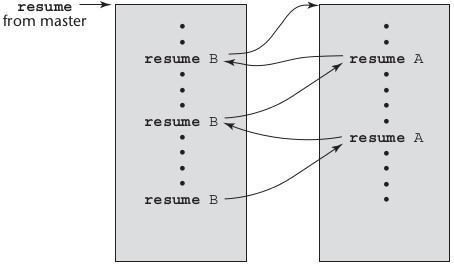
\includegraphics[scale=0.5]{./imgs/coroutines.png}
\label{co-rotinas}
\end{figure}
\end{frame}

\begin{frame}{Co-rotinas}
\begin{figure}[ht!]
 \centering
 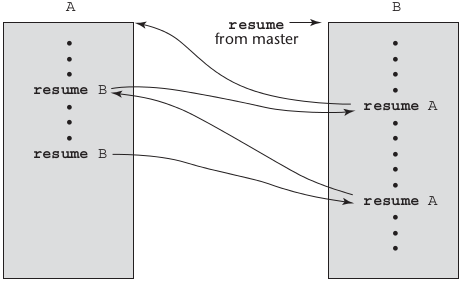
\includegraphics[scale=0.5]{./imgs/coroutines_b.png}
\label{co-rotinas_b}
\end{figure}
\end{frame}




\end{document}